\documentclass[a4paper,11pt,fleqn,twoside,openright]{memoir} % Brug openright hvis chapters skal starte på højresider; openany, oneside

%%%% PACKAGES %%%%

%  Oversættelse og tegnsætning  %
\usepackage[utf8]{inputenc}					% Gør det muligt at bruge æ, ø og å i sine .tex-filer
%\usepackage[danish]{babel}							% Dansk sporg, f.eks. tabel, figur og kapitel
\usepackage[english]{babel}
\usepackage[T1]{fontenc}  % Hjælper med orddeling ved æ, ø og å. Sætter fontene til at være ps-fonte, i stedet for bmp					
\usepackage{latexsym}										% LaTeX symboler
\usepackage{xcolor,ragged2e,fix-cm}			% Justering af elementer
\usepackage{pdfpages} % Gør det muligt at inkludere pdf-dokumenter med kommandoen \includepdf[pages={x-y}]{fil.pdf}	
\usepackage{fixltx2e}					% Retter forskellige bugs i LaTeX-kernen

																			
%  Figurer og tabeller floats %
\pdfoptionpdfminorversion=6	% Muliggør inkludering af pdf dokumenter, af version 1.6 og højere
\usepackage{graphicx} 		% Pakke til jpeg/png billeder
	
%  Matematiske formler og maskinkode 
\usepackage{amsmath,amssymb,stmaryrd} 	% Bedre matematik og ekstra fonte
\usepackage{textcomp}                 	% Adgang til tekstsymboler
\usepackage{mathtools}			% Udvidelse af amsmath-pakken.
\usepackage{siunitx}			% Flot og konsistent præsentation af tal og enheder med \SI{tal}{enhed}

%  Referencer, bibtex og url'er  %
\usepackage{url}	% Til at sætte urler op med. Virker sammen med hyperref
%\usepackage[danish]{varioref} % Giver flere bedre mulighed for at lave krydshenvisninger
\usepackage[english]{varioref} % Giver flere bedre mulighed for at lave krydshenvisninger
\usepackage{natbib}	% Litteraturliste med forfatter-år og nummerede referencer
\usepackage{xr}		% Referencer til eksternt dokument med \externaldocument{<NAVN>}
\usepackage{nomencl}	% Pakke til at danne nomenklaturliste
\makenomenclature		% Nomenklaturliste

%  Floats  %
\let\newfloat\relax 	% Memoir har allerede defineret denne, men det gør float pakken også
\usepackage{float}
%\usepackage[footnote,draft,danish,silent,nomargin]{fixme}	% Indsæt rettelser og lignende med \fixme{...} Med final i stedet for draft, udløses en error for hver fixme, der ikke er slettet, når rapporten bygges.
\usepackage[footnote,draft,english,silent,nomargin]{fixme}

%%%% CUSTOM SETTINGS %%%%

%  Marginer  %
\setlrmarginsandblock{3.5cm}{2.5cm}{*}	% \setlrmarginsandblock{Indbinding}{Kant}{Ratio}
\setulmarginsandblock{2.5cm}{3.0cm}{*}	% \setulmarginsandblock{Top}{Bund}{Ratio}
\checkandfixthelayout 

%  Litteraturlisten  %
\bibpunct[,]{[}{]}{;}{a}{,}{,} 	% Definerer de 6 parametre ved Harvard henvisning (bl.a. parantestype og seperatortegn)
\bibliographystyle{bibtex/harvard}	% Udseende af litteraturlisten. Ligner dk-apali - mvh Klein

%  Indholdsfortegnelse  %
\setsecnumdepth{subsection}	% Dybden af nummerede overkrifter (part/chapter/section/subsection)
\maxsecnumdepth{subsection}	% Ændring af dokumentklassens grænse for nummereringsdybde
\settocdepth{subsection} 		% Dybden af indholdsfortegnelsen


%  Visuelle referencer  %
\usepackage[colorlinks]{hyperref} % Giver mulighed for at ens referencer bliver til klikbare hyperlinks. .. [colorlinks]{..}
%\usepackage{memhfixc}
\hypersetup{pdfborder = 0 0 0}	% Fjerner ramme omkring links i fx indholsfotegnelsen og ved kildehenvisninger 
\hypersetup{			%	Opsætning af farvede hyperlinks
    colorlinks = false,
    linkcolor = black,
    anchorcolor = black,
    citecolor = black
}

\definecolor{gray}{gray}{0.80}					% Definerer farven grå

%  Kapiteludssende  %
\definecolor{numbercolor}{gray}{0.7}			% Definerer en farve til brug til kapiteludseende
\newif\ifchapternonum

\makechapterstyle{jenor}{			% Definerer kapiteludseende -->
  \renewcommand\printchaptername{}
  \renewcommand\printchapternum{}
  \renewcommand\printchapternonum{\chapternonumtrue}
  \renewcommand\chaptitlefont{\fontfamily{pbk}\fontseries{db}\fontshape{n}\fontsize{25}{35}\selectfont\raggedleft}
  \renewcommand\chapnumfont{\fontfamily{pbk}\fontseries{m}\fontshape{n}\fontsize{1in}{0in}\selectfont\color{numbercolor}}
  \renewcommand\printchaptertitle[1]{%
    \noindent
    \ifchapternonum
    \begin{tabularx}{\textwidth}{X}
    {\let\\\newline\chaptitlefont ##1\par} 
    \end{tabularx}
    \par\vskip-2.5mm\hrule
    \else
    \begin{tabularx}{\textwidth}{Xl}
    {\parbox[b]{\linewidth}{\chaptitlefont ##1}} & \raisebox{-15pt}{\chapnumfont \thechapter}
    \end{tabularx}
    \par\vskip2mm\hrule
    \fi
  }
}			% <--

\chapterstyle{jenor}	% Valg af kapiteludseende - dette kan udskiftes efter ønske


%\renewcommand{\headrulewidth}{0.4pt}
%\renewcommand{\footrulewidth}{0.4pt}


% Sidehoved %

\makepagestyle{custom} % Definerer sidehoved og sidefod - kan modificeres efter ønske -->
\makepsmarks{custom}{																						
\def\chaptermark##1{\markboth{\itshape\thechapter. ##1}{}} % Henter kapitlet den pågældende side hører under med kommandoen \leftmark. \itshape gør teksten kursiv
\def\sectionmark##1{\markright{\thesection. ##1}{}}	% Henter afsnittet den pågældende side hører under med kommandoen \rightmark
} % Sidetallet skrives med kommandoen \thepage	
\makeevenhead{custom}{Gruppe B205}{}{} % Definerer lige siders sidehoved efter modellen \makeevenhead{Navn}{Venstre}{Center}{Højre}
\makeoddhead{custom}{}{}{Aalborg Universitet} % Definerer ulige siders sidehoved efter modellen \makeoddhead{Navn}{Venstre}{Center}{Højre}
\makeevenfoot{custom}{Page \thepage}{}{}													% Definerer lige siders sidefod efter modellen \makeevenfoot{Navn}{Venstre}{Center}{Højre}
\makeoddfoot{custom}{}{}{Page \thepage}														% Definerer ulige siders sidefod efter modellen \makeoddfoot{Navn}{Venstre}{Center}{Højre}		
\makeheadrule{custom}{\textwidth}{0.5pt}	 % Tilføjer en streg under sidehovedets indhold
\makefootrule{custom}{\textwidth}{0.5pt}{1mm}	% Tilføjer en streg under sidefodens indhold

\copypagestyle{nychapter}{custom}														% Følgende linier sørger for, at sidefoden bibeholdes på kapitlets fåøste side
\makeoddhead{nychapter}{}{}{}
\makeevenhead{nychapter}{}{}{}
\makeheadrule{nychapter}{\textwidth}{0pt}
\aliaspagestyle{chapter}{nychapter}													% <--

\pagestyle{custom} % Valg af sidehoved og sidefod


%%%% CUSTOM COMMANDS %%%%

%  Promille-hack (\promille)  %
\newcommand{\promille}{%
  \relax\ifmmode\promillezeichen
        \else\leavevmode\(\mathsurround=0pt\promillezeichen\)\fi}
\newcommand{\promillezeichen}{%
  \kern-.05em%
  \raise.5ex\hbox{\the\scriptfont0 0}%
  \kern-.15em/\kern-.15em%
  \lower.25ex\hbox{\the\scriptfont0 00}}

% Billede hack %
\newcommand{\figur}[4]{
		\begin{figure}[H] \centering
			\includegraphics[width=#1\textwidth]{billeder/#2}
			\caption{#3}\label{#4}
		\end{figure} 
}

%%%% ORDDELING %%%%

\hyphenation{hvad hvem hvor}

\begin{document}	% Starter dokumentet - obligatorisk

\frontmatter % Forindhold - nummereres med romertal

\thispagestyle{empty}
\begin{flushright}
\vspace{3cm}

\phantom{hul}

\phantom{hul}

\phantom{hul}

\textsl{P2 Project} \\ \vspace{1cm}

\rule{13cm}{3mm} \\ \vspace{1.5cm}
\vspace{1cm}

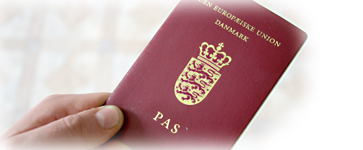
\includegraphics[width=0.4\textwidth]{billeder/forside.jpg}

\vspace{2cm} 
\textsc{\Large Bag Packer \\
P2 project\\
Group B130\\
Software\\
Department of Computer Science\\
Aalborg University\\
The 24th of May 2012\\
}
\end{flushright}

\cleardoublepage % Indsætter tom side (hvis nødvendigt)

% Dette er LaTeX-versionen af titelbladet for tek-nat-basis-rapporter 2004 efterår
% Filen kræver:
% Universitetets logo:  aau-logo.png (for LaTeX) eller aau-logo.ps (for LaTeX)
% Synopsis: En fil ved navn synopsis.tex

% Udarbejdet af: Hans Hüttel (hans@cs.auc.dk) 21. maj 2003
% Rettet af Morten Christophersen (mortench@tnb.aau.dk) 30. nov 2004(ændret til nyt design 2004 efterår)

%\documentclass[11pt]{article}
%\ifx\pdfoutput\undefined 
%\usepackage[dvips]{graphicx}
%\else
%\usepackage[pdftex]{graphicx} 
%\usepackage{type1cm} \fi
  %  \usepackage[ansinew]{inputenc}
    %\usepackage{a4}

%\begin{document} 
%\thispagestyle{empty}
%\begin{titlepage}

\begin{nopagebreak}
{\samepage 
\begin{tabular}{r}
\parbox{\textwidth}{  \raisebox{11mm}{
\includegraphics[height=1cm]{billeder/aaulogo.jpg}}
\hfill \parbox{8cm}{\begin{tabular}{l}
{\small \textbf{Faculty Office for Engineering and Science }}\\
{\small Strandvejen 12-14} \\
{\small Phone 96 35 97 31} \\
{\small Fax 98 13 63 93} \\
{\small http://tnb.aau.dk}
\end{tabular}}}
\\
\end{tabular}

\begin{tabular}{cc}
\parbox{7cm}{
\begin{description}

\item {Title:} 

Passport photo program
  
\item {Theme:} 

Programmatic image editing

\end{description}

\parbox{8cm}{

\begin{description}
\item {Project period:}\\
   P1, fall 2011\\
  \hspace{4cm}
\item { Project group:}\\
  B205\\
  \hspace{4cm}
\item { Participants:}\\
Dag Toft Børresen Pedersen \\
Christian Jødal O'Keeffe \\
Niels Brøndum Pedersen \\
Aleksander Sørensen Nilsson \\
Mette Thomsen Pedersen \\
Rasmus Fischer Gadensgaard \\
Kasper Plejdrup\\
  \hspace{2cm}
\item { Supervisor:}\\
Karsten Jahn\\
\item { Secondary supervisor:}\\
Marion Berg Christiansen\\
\end{description}
}
\begin{description}
%\item { Total number of pages:} \pageref{VeryLastPage}
\item { Finished: } 20/12-2011
\end{description}
\vfill } &
\parbox{7cm}{
  \vspace{.15cm}
  \hfill 
  \begin{tabular}{l}
  { Synopsis:}\bigskip \\
  \fbox{
    \parbox{6.5cm}{\bigskip
     {\vfill{\small This report contains documentation of which problems some people might have packing their suitcases before a flight travel. These chapters will lead up to a statement of the problem which will be used in the development of a solution.
\newline
The solution will be a program based on the programming language C#. There will be a chapter describing how the structure of the program will be, and the reason behind the construction. There will also be a section about the reflections made, when the program was being made.
\newline
One of the last chapters will concern the testing and conclusion of the finished program. What could have been done better to the program and why does it not work, if that is the case. This chapter will also concern the reflection on the product to see if it actually solves the problem or why it does not solve the problem.
\newline
The product of the project is a program that helps the user pack a suitcase efficiently, and through a 3D-image of the packed suitcases the user will see where in the suitcase each item must be put.
     \bigskip}}
     }}
   \end{tabular}}
\end{tabular}}
\\ \\

\begin{description}
\item { Source of front page picture:}\\
http://www.frederiksberg.dk/Borgerservice/PasOgKoerekort/Pas.aspx\\
\end{description}

\noindent{\footnotesize\emph{The content of the report is freely available, but can only be published (with source reference) with an agreement with the authors.}}
\end{nopagebreak}
%\end{titlepage}
%\end{document}

\cleardoublepage
Date:\indent\indent Aleksander Sørensen Nilsson\\\\\\
\indent\line(1,0){200}\\\\\\
\indent Date:\indent\indent Christian Jødal O'Keefe\\\\\\
\indent\line(1,0){200}\\\\\\
\indent Date:\indent\indent Dag Toft Børresen Pedersen\\\\\\
\indent\line(1,0){200}\\\\\\
\indent Date:\indent\indent  Kasper Plejdrup\\\\\\
\indent\line(1,0){200}\\\\\\
\indent Date:\indent\indent  Mette Thomsen Pedersen\\\\\\
\indent\line(1,0){200}\\\\\\
\indent Date:\indent\indent  Niels Brøndum Pedersen\\\\\\
\indent\line(1,0){200}\\\\\\
\indent Date:\indent\indent  Rasmus Fischer Gadensgaard\\\\\\
\indent\line(1,0){200}\\\\\\

\cleardoublepage
\chapter{Forord}
\cleardoublepage

%%%% Indholdsfortegnelse (TOC) %%%%


\setlength\parskip{0ex} % Fjerner den vertikale afstand mellem hver linie i indholdsfortegnelse
\tableofcontents* % Indholdsfortegnelsen 
\setlength{\parskip}{3mm} % Aktiverer afstanden igen for resten af rapporten (afstem med preamble!)

%\addtocontents{toc}{\protect\newpage} % Fremtvinger sideskift i indholdsfortegnelsen hvis nødvendig


\label{marker}
\mainmatter

 % Hovedindhold - nummereres fra side 1
\makeevenfoot{custom}{Page \thepage~of \pageref{LastPage}}{}{}	% Definerer lige siders sidefod efter modellen \makeevenfoot{Navn}{Venstre}{Center}{Højre}
\makeoddfoot{custom}{}{}{Page \thepage~of \pageref{LastPage}}% Definerer ulige siders sidefod efter modellen \makeoddfoot{Navn}{Venstre}{Center}{Højre}		
\pagestyle{custom}


%%%% Rapportindhold %%%%
\chapter{Introduction} 
This project is based on the subject "image editing" with a focus on passport photos. From this project a product should emerge that will try and deal with a problem within the subject's field. When the product is done, it should be tested and based on the test it will be possible to evaluate the product's capability at solving the problem.
\newline
It is a requirement that the program is made in the program language C. The program will therefore be a command line based program.\newline
A part of the project is to document a problem and analyse it, to find the reason behind the problem. When the analysis is done, the product should be designed to handle the problem and thus solve it.
\newline
This is the essential of problem-based learning: to find a problem and then solve it and hopefully gaining some knowledge in the process.
For this to be an effective model all the group members must participate in the process and acquire knowledge by working with the project.
\chapter{Problem Analysis}
\input{indhold/problemanalysis/Introduction.tex}
\input{indhold/problemanalysis/Whywehavepassports.tex}

\input{indhold/problemanalysis/Biometricpassphoto.tex}
\input{indhold/problemanalysis/Requirementstophoto.tex}
\input{indhold/problemanalysis/Problemswithphotos.tex}
\input{indhold/problemanalysis/Otherpassportphotoprograms.tex}
\input{indhold/problemanalysis/Thesisstatement.tex}
\input{indhold/problemanalysis/Method.tex}

\chapter{Theory}
In this chapter a closer look will be taken on the theoretical aspect of writing a sorting program.
With a good grasp on the different algorithms and the most effective way to pack items, the process of developing a program should be easier. A famous packing problem is the Knapsack problem, which is described in detail in section \ref{sec:knapsack}. A derivative of the Knapsack problem is the bin packing problem, which is described in section \ref{sec:binpacking}.
\input{indhold/theory/Photoeditingthroughtime.tex}
\input{indhold/theory/Imageeditingtoday.tex}
\input{indhold/theory/Photoanalysis.tex}
\input{indhold/theory/Librariescomparison.tex}
\input{indhold/theory/Libjpeg.tex}
\input{indhold/development/Pixeltoinch.tex}

\chapter{Design}
\input{indhold/design/Introdesign.tex}
\input{indhold/problemanalysis/Targetgroupanalysis.tex}
\section{Specification Requirements}
\label{sec:Spec}
Through the problem analysis it has been documented that there are some strict rules regarding some forms of public transportation when going on vacation. Based on this research a list of features have been composed, that the program must fulfil to meet the base requirements.
Furthermore another list have also been made composed of some additional features that would make the program better and more user friendly. They are not needed for the base requirements, but rather as improvements to further make the program ideal for the user.

For the user to better get started on the program there will be a guide that come with the program. The guide gives an explanation on how to use the program. The guide will be short and well formulated so the user with ease can read and understand the guide.
The project description states that the program language must be written in C#.
The program itself needs to have a few features for it to solve the problem that is the focus of this project. The program needs to make sure that the weight is evenly distributed in the bags and that it does not exceed the bags weight limits. The program also needs to distribute the space of the bags to make sure that the program does not fill a bag more than there is physical room for.
When the user is on the trip the program needs to have a function that allows the user to edit the list over items that are in the bag so if the user buys some souvenirs or throws something away, the list of items will be updated and thereby a new way to pack the luggage.
The program will need a function to help the user see where the items are placed in the luggage.
The program will also have to check that the suitcases are below the limits set for weight and size.


There are some features that not are essential for the program to work but will improve the program. One of these features is to handle changeable shape of items e.g. a T-shirt or other forms of clothing. This makes the program able to pack more efficient. This mean that to program can handle like solid, liquid and bendable shapes. But this may not be in the program at the start since this will be hard to develop and implement.
To better help packing and planing ahead the program needs a list of different trip types that can help the user with packing the luggage for a given type of trip.
Another nice feature to have is to save space for possible souvenirs the user might buys on the trip. These features means that the user does not need to check if there is room for the souvenirs before buying it.

\subsection{Targeted Features}
These are the essential features that the program will have.\newline

\textbf{program language is C#}:
The program need to written in C# since the requirements for this project is that the program need to written in C#.

\textbf{Guide the user}:
The program will have a little "readme" file, or other form of guide, that will tell the customer how to use the program.
\newline

\textbf{Distribute weight}:
The program must be able to distribute weight of items evenly in each individual suitcase and if needed spread out in multiple suitcases.
\newline

\textbf{Distribute space}:
The program also needs to distribute the items by space. The whole idea of the program, is that it should be able to tell the user how to pack the suitcase, and be able to tell if there is enough space for eventual souvenirs. Lastly it should inform the user how much space, if any, is left.
\newline

\textbf{On the road}:
The program will be able to tell you, while you are on the trip, if there is enough space for a souvenirs, if you input the dimensions and weight of that item. And if you what to remove a item from your luggage the it can this as well.
\newline

\textbf{Baggage rules}:
The program will need to know basic baggage rules. For example the luggage must not weigh too much, and it must be below certain dimensions.
\newline

\textbf{Structure of packing}:
When the user asks the program if an item will fit in the suitcase, the program will show exactly where in the suitcase the item will fit.
\newline

\textbf{Packing list}:
To make it easier for the user to know what will be packed an editable lists will be included depending on the type of trip.
\newline

\textbf{Number of people}
Usually a trip is done with more then one person, so more suitcases might be available to distribute items between.
\newline

\subsection{Optional Features}
These features as mentioned above, are additional features that might be able to be implemented later if possible.\newline

\textbf{Solid/liquid/bendable shapes}:
The program will also take in account that items might be bendable, and therefore fit in other ways than solid items. For instance a T-shirt can be folded in many ways and thus can be considered a liquid form as it can fit almost everywhere.
\newline

\textbf{Type of trip}
Depending on the nature of the trip different packing lists will be necessary because each trip might require different items.
\newline

\textbf{Account for the trips length}:
If a long trip is planned, the program can take in account that the user might need more space for souvenirs, so the user do not need to check on the trip if there is room and weight for every souvenirs in the luggage and decide if the souvenir can come in the luggage without exceed the weight limit.
\newline
\input{indhold/problemanalysis/Problemsolution.tex}
\input{indhold/design/Programplanning.tex}


\chapter{Development}
\input{indhold/development/Forwordtoprogramdecription.tex}
\input{indhold/development/Descriptionofthescalingmarks.tex}
\input{indhold/development/Findingthehead.tex}
\input{indhold/development/Markhead.tex}
\input{indhold/development/Funktiontilkorrektforhold.tex}
\input{indhold/development/FunktiontilatberegneDPI.tex}
\input{indhold/development/Lightdarkfunc.tex}
\input{indhold/development/Functioncrop.tex}
\input{indhold/development/Askingandgettinganswer.tex}

\input{indhold/development/Instructionmanual.tex}


\chapter{Testing} 
\input{indhold/testing/Purposeoftesting.tex}
\input{indhold/testing/Testperson.tex}
\input{indhold/testing/Choiceofsurveymethodandwhyuseit.tex}
\input{indhold/testing/Testoftheprogram.tex}
\input{indhold/testing/Secondtestoftheprogram.tex}

\chapter{Discussion}
\input{indhold/discussion/Introtodiscussion.tex}
\section{Discussion}
The focus in this discussion is to see if the product is in conjunction with the problem analysis and to see if the different requirements is integrated in the product.

In the problem analysis there was stated the following requirements for the program:

\begin{itemize}
\item Program language is C\#.
\item Guide the user.
\item Distribute weight.
\item Distribute space.
\item On the road.
\item Baggage rules.
\item Structure of packing.
\item Packing list.
\item save/load function.
\end{itemize}

And there also were some Optional Features that if there where time left those might be implemented in the program:
\begin{itemize}
\item Solid/liquid/bendable shapes.
\item Type of trip.
\end{itemize}

The program is based on the requirements and has been improved using the tests that have been made on the program. The tests have helped with improving the design of the program and a few function in the program. This has been a very good tool in improving and bug-testing the program. The improvement made after the tests can be seen in chapter \ref{chap:testing}.

In section \ref{sec:devalgorithm} the algorithm are explained. The algorithm distribute the items in the suitcase(s) evenly by weight and space. The algorithm also make sure that the weight limit is not exceeded. Yet the algorithm can not pack as good as a person might be able to do. One reason that a person might be better at packing the suitcase,, is that the program take all the items as boxes and do not take into account, that some items might be able to be fold and bend in different shapes.

To help the user to get a better visual understanding on how to pack the suitcase a 3D-image is made for the user that can rotate, zoom and be dragged. A list has been added in the right side showing a list of all the packed items in the selected suitcase. By selecting an item it will be marked in the 3D-image so the user will easily be able to identify any given item. An explanation of this function can be seen in section \ref{3DHandle}. To help the user furthermore an algorithm has been made that makes sure that any two items next to each other will have different colors, so they are easier to identify from each other. The function and a description of it can be seen in section \ref{sec:ColorGiver}.

It is easy to get a good overview in the program, because the maximum number of buttons is 5 in all the different windows and no unnecessary features are in the windows. The 3D-viewer is very user friendly because the user can use the mouse to zoom and rotate the 3D-image of the suitcase containing the packed items. The section where the GUI is described is in section \ref{sec:GUI}.

The user are able to save a list he/she has made on the computer and load saved list every time he/she uses the program.

\fxfatal{det der står under skal skrived om på.}
-------------------------------------------------------------------------- 

The user can make or save into a file that also can be loaded by the program to get the data that are in the file. There is different way to save data one is to use windows SQL database that where not ideally because it need a SQL handling program or internet connection to use. Therefore there is use a File serializer that make a file with the data. This is useful because it make it easily to choose where the data should be save into the data file or with data file should be load into the program.
\section{Perspectivation}
When working with problem solving it is also important to look at how the user will use and interact with the solution. Through these assumptions a better solution can be formed that is more user friendly. Therefore it is a good thing to know who are going to use the solution, and from that design it more thoughtfully.

The purpose in this project was to make a program that provided the user with a packing solution and help the users pack a suitcase more effectively. The program should also check that the weight of the suitcase does not exceed the limits given by the user. The program is made in Microsoft Visual Studio that provides the developer with a lot of good tools to make a user interface for the user of the program.
This makes the program a lot more user friendly because the user can easier interact with the program. This means that it will be a lot easier for the user to operate the program and thereby the program have bigger chance to sell if it were the intention.
The user interface also means that the user does not need to understand the program before they can use it.
The program in this project also supports mouse control, this means that the user can use a mouse to navigate around the program. Because of the mouse support, and the interface the user has less of a risk to something wrong when using the program, but by implementing an interface there is a risk for new bugs and misunderstandings in the formulations of the interface.
Therefore it is important to make a clean and user friendly interface that only contains the necessary buttons and well formulated text that helps the user by informing about what they should do, and what kind of unit the data is measured in.

To prepare the program and try to find potential problems, the program has undergone some tests, where people who have not worked with the project have tried the program. Their experiences from the test were then collected and used to evaluate the program. The evaluation then led to changes that would make the program better. After the changes were made, the program were tested again with the changes and the same procedure of the test result as the earlier test.
This process of repeated testing is a good procedure to develop a working program because the potential user gets to use it and experiences are made in context to the use. These experiences are then used to make the program more suited for the target audience. The downside of this procedure is that it takes a lot of man hours to do the testing and make the changes. Therefore testing is a good but expensive tool, hour-wise, to use.
It should always be taken into consideration to test the program, because it is important that the program is freed of the worst bugs when released. Program bugs on releases have a negative influence on the programs sale and might scare of potential purchasers.

A side effect from making the program in Visual Studio is that the program only can run on Microsoft Windows with the .NET framework installed. The reason for this is that the program uses the .NET framework which only supports Microsoft's operating systems.
This means that it is important to take a moment before developing and make a thought regarding what platform the program should be used on or better yet, if it should be able to run cross platforms.
These different experiences made in this project can be used in upcoming projects.

The program, when used correctly, can help one person with a lot of suitcases or groups of people pack their luggage pretty effectively among all their suitcases. Furthermore, the program can help make sure that the user is not exceeding the weight limit, if any, for the given trip provided that the user knows the limit. This can save the user the burden of additional work and financing due to overweight and thus improve the overall experience of the trip as well as improve the environment because of the reduced weight to the transport vehicles. When the user saves money because they avoided the overweight fee, they might use that money on the resort and thus help the given country they are visiting. This can have a positive impact on that country's resorts giving them more money they can use to improved their facilities.

The final chapter of the report is a conclusion on the whole project and a conclusion on the problem statement.

To make a conclusion on this project it is necessary to take a closer look on the problem statement, see section \ref{sec:thesis}. To meet and answer the problem statement, the program must be able to pack one or more suitcases by volume and weight in an effective way. It is also required that the program must present the result to the user in some way before it actually can help the user.

The program is capable of packing one or more suitcases with items while using the volume as effectively within the programs reach. When mentioning the program reach is that program handles the items as boxes instead of their real shape.
The program does not pack as effectively as possible because that will include that the program treats items as different objects and not just boxes. The program also distribute the weight evenly among the suitcases if there is more than one and checks if that the suitcases do not exceed a given limit. The program also have an user interface that fulfills the role as deliver of the result.

The program gives a packing solution but not as effectively as possible and thereby the program itself does not give an fully answer to the problem statement. The answer should be find through experience and knowledge gained in this project. The reason for this is that with new knowledge it will be possible to take this program and improve it so program better handles the items that should be packed. So for the program to be able to pack more effectively it must be better at handle all kind of shapes and be able place them compared to each other.

So it can be conclude that problem statement have been answered through the work the final product but the problem statement is not answered that the product itself. The reason is that the program only gives the most effective packing solution within the criterion that items is handle as boxes.

The program also solves the problem stated in the project suggestion, about making a program able to help with planning how to pack a suitcase (see appendix \ref{chap:forslag}. It can be concluded that the program can pack one or more suitcases using weight distributing. It might be improved by a function that handles bendable shapes, but even though the program is missing that feature it is able to pack one or more suitcases in a good and efficient way. Therefore it is a good program that helps the user with the process of packing one or more suitcases while using weight distributing but it could be improved if more time were available.

%The program has been written in the programming language C\# and a user interface has been made to make it easier for the user to use the program. When opening the program the main window of the program will appear. Here the instructions on how to use the program will be shown so the user always have them at hand. From the main window the user can either get informations about the creators of the program, load a previous saved list, manage the lists or start the packing. The program saves the lists on the computer a user specified path. This means the program can be used at any time even without an Internet connection. 

%In the manage windows the user can see the list of added suitcases or items and be able to edit the list. The user will be able to add new items or suitcases to the list, delete items or suitcases or edit already made items or suitcases. The user will have to provide the program with the items dimensions and weight and when adding suitcases also the weight limit for the suitcase. From the manage windows the user can save the lists on the computer for later use. 

%After the users are done managing the lists the user is returned to the main window where a button will start the algorithm managing the packing. When the algorithm is done a window will appear showing a 3D-image of the suitcase with all the things to be packed inside. A list of the items will be on the right side and when an item is selected it will be highlighted in the 3D-image. The image can be dragged, rotated and zoomed so the user have the best possibilities to view the 3D-image as he/she wants.

%The program covers the targeted requirements for the product and therefore the program solves the problem stated in the problem statement.

%%%% Kilder %%%%

\begingroup
	\raggedright
	\bibliography{bibtex/litteratur}	% Litteraturlisten
\endgroup

%%%% Fixme-listen %%%%

%\newpage
%\listoffixmes	% Fixme-listen - fjernes til sidst i projektet med "%"

\clearforchapter
\appendix	% Appendiks/bilag start - giver chapter bogstaver i stedet for tal

\aliaspagestyle{chapter}{empty}	 % Fjernelse af nummerering på bilagenes chaptersider
\pagestyle{empty}	%	Fjernelse af nummerering i bilag
\addtocontents{toc}{\protect\cftpagenumbersoff{chapter}} % Fjernelse af nummerering af bilag i TOC

%\settocdepth{chapter}	% Sætter dybden af indholdsfortegnelsen til chapter for bilagene


%%%% Appendiks %%%%
\section{Questionnaire}

1. Were there some problems with finding out how the program worked?

2. Were there were some technical problems by using the program?

3. Other problems?

4. The program was easy to use?

5. How was designed of the program?

6. Did you find the program helpful?

7. Would you use a similar program?

8. Suggestions for improvements?

9. Other comments?
\input{indhold/appendix/Mindmap.tex}
\input{indhold/appendix/projektforslag.tex}
%%%% Bilag %%%%

\end{document}																								% Slutter dokumentet - obligatorisk


